\documentclass[tikz,border=14pt]{standalone}
\usepackage{tikz}
\usepackage{amsmath}
\usetikzlibrary{positioning,fit,arrows.meta,calc,backgrounds}

% ── Colour palette ──────────────────────────────────────────────────────────
\definecolor{stateBlue}{HTML}{2E86AB}      % hidden states
\definecolor{obsGreen}{HTML}{3BB273}       % observations
\definecolor{transOrange}{HTML}{E84855}    % transition arrows
\definecolor{emitPurple}{HTML}{7B2D8B}     % emission arrows
\definecolor{plateGray}{HTML}{AAAAAA}      % plate border
\definecolor{annoTrans}{HTML}{C0392B}      % transition annotation text
\definecolor{annoEmit}{HTML}{6C3483}       % emission annotation text
\definecolor{colL}{HTML}{E41A1C}           % histogram bar left
\definecolor{colC}{HTML}{377EB8}           % histogram bar centre
\definecolor{colR}{HTML}{4DAF4A}           % histogram bar right
\definecolor{colTA}{HTML}{E41A1C}          % trans bar 1 – red
\definecolor{colTB}{HTML}{FFC107}          % trans bar 2 – amber
\definecolor{colTW}{HTML}{0078D4}          % trans bar k – windows blue

\begin{document}
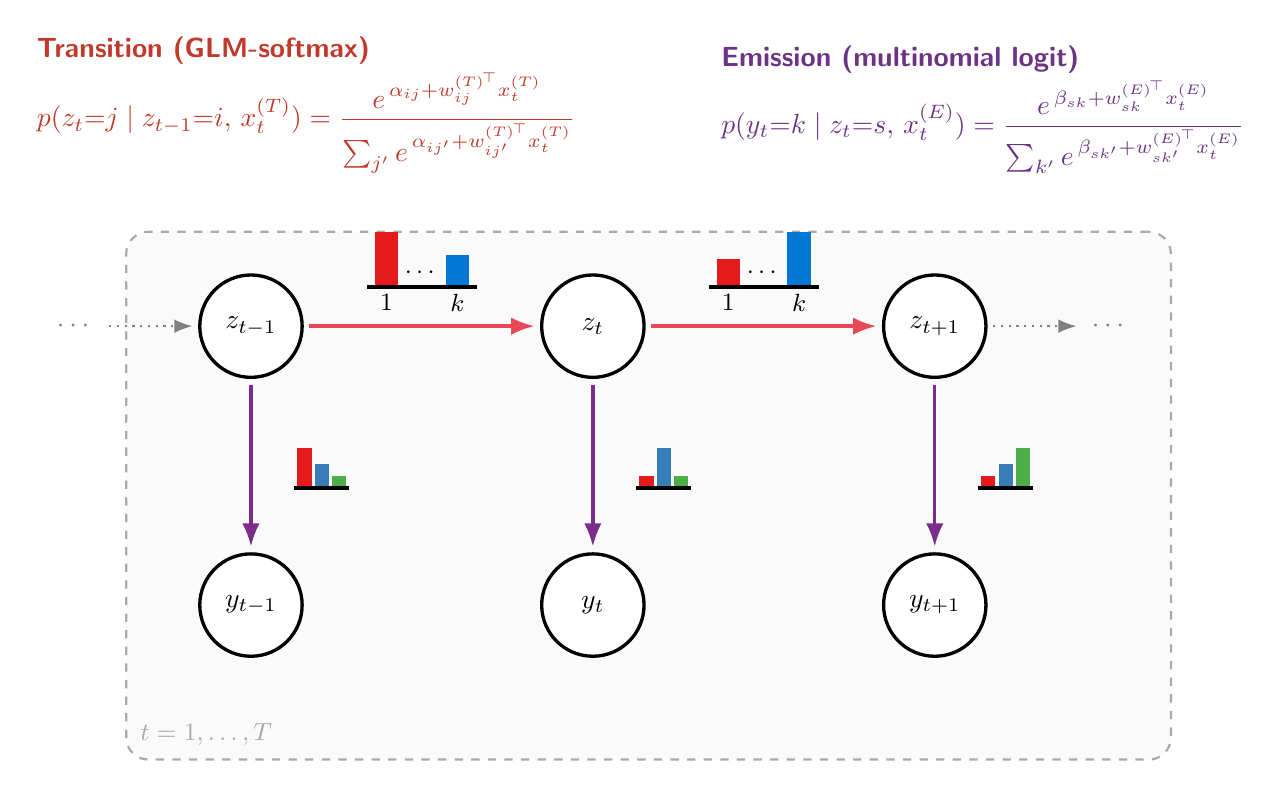
\begin{tikzpicture}[
  font=\sffamily,
  >=Latex,
  %% Node styles
  state/.style={
    circle, draw=black, fill=white,
    very thick, minimum size=13mm, inner sep=0pt,
    font=\sffamily\bfseries
  },
  obs/.style={
    circle, draw=black, fill=white,
    very thick, minimum size=13mm, inner sep=0pt,
    font=\sffamily\bfseries
  },
  %% Arrow styles
  tarrow/.style={->, very thick, color=transOrange,
                 shorten >=2pt, shorten <=2pt},
  earrow/.style={->, very thick, color=emitPurple,
                 shorten >=2pt, shorten <=2pt},
  dotarrow/.style={->, thick, dotted, color=black!50,
                   shorten >=2pt, shorten <=2pt},
]

%% ── Hidden states ──────────────────────────────────────────────────────────
\node[state] (z0) {$z_{t-1}$};
\node[state, right=30mm of z0] (z1) {$z_t$};
\node[state, right=30mm of z1] (z2) {$z_{t+1}$};

%% entry / exit dots
\node[left=12mm  of z0, text=black!50] (ldots) {$\cdots$};
\node[right=12mm of z2, text=black!50] (rdots) {$\cdots$};

%% ── Observations ───────────────────────────────────────────────────────────
\node[obs, below=22mm of z0] (y0) {$y_{t-1}$};
\node[obs, below=22mm of z1] (y1) {$y_t$};
\node[obs, below=22mm of z2] (y2) {$y_{t+1}$};

%% phantom nodes to push plate borders
\node[below=7.5mm of y1, inner sep=0pt, minimum size=0pt] (phantomBot) {};
\node[right=14mm of y2,  inner sep=0pt, minimum size=0pt] (phantomRight) {};

%% ── Transition arrows ──────────────────────────────────────────────────────
\draw[dotarrow] (ldots) -- (z0);
\draw[tarrow]   (z0)    -- (z1);
\draw[tarrow]   (z1)    -- (z2);
\draw[dotarrow] (z2)    -- (rdots);

%% ── Transition bar-plots (above red arrows) ─────────────────────────────
%% Each mini-histogram: bar_1 (red), ···, bar_k (windows blue), "k" below bar k
%% ─ above z0→z1: state-1-heavy distribution
\coordinate (ht0) at ($(z0)!0.5!(z1)+(0,8mm)$);
\fill[colTA] ($(ht0)+(-6mm,-3mm)$) rectangle ($(ht0)+(-3mm, 4mm)$);
\fill[colTW] ($(ht0)+(3mm,-3mm)$)  rectangle ($(ht0)+(6mm,  1mm)$);
\draw[black, line width=1.3pt] ($(ht0)+(-7mm,-3mm)$) -- ($(ht0)+(7mm,-3mm)$);
\node[font=\sffamily\small] at ($(ht0)+(0,-1.2mm)$) {$\cdots$};
\node[font=\sffamily\small] at ($(ht0)+(-4.5mm,-5mm)$) {$1$};
\node[font=\sffamily\small] at ($(ht0)+(4.5mm,-5mm)$)  {$k$};

%% ─ above z1→z2: state-k-heavy distribution
\coordinate (ht1) at ($(z1)!0.5!(z2)+(0,8mm)$);
\fill[colTA] ($(ht1)+(-6mm,-3mm)$) rectangle ($(ht1)+(-3mm,  0.5mm)$);
\fill[colTW] ($(ht1)+(3mm,-3mm)$)  rectangle ($(ht1)+(6mm,  4mm)$);
\draw[black, line width=1.3pt] ($(ht1)+(-7mm,-3mm)$) -- ($(ht1)+(7mm,-3mm)$);
\node[font=\sffamily\small] at ($(ht1)+(0,-1.2mm)$) {$\cdots$};
\node[font=\sffamily\small] at ($(ht1)+(-4.5mm,-5mm)$) {$1$};
\node[font=\sffamily\small] at ($(ht1)+(4.5mm,-5mm)$)  {$k$};

%% ── Emission arrows ────────────────────────────────────────────────────────
\draw[earrow] (z0) -- (y0);
\draw[earrow] (z1) -- (y1);
\draw[earrow] (z2) -- (y2);

%% ── Histograms beside emission arrows (right side) ──────────────────────────
%% y0: left-skewed  (tall L, medium C, short R)
\coordinate (h0) at ($(z0)!0.5!(y0)+(9mm,0)$);
\fill[colL] ($(h0)+(-3.1mm,-2.8mm)$) rectangle ($(h0)+(-1.3mm, 2.2mm)$);
\fill[colC] ($(h0)+(-0.9mm,-2.8mm)$) rectangle ($(h0)+(0.9mm,  0.2mm)$);
\fill[colR] ($(h0)+(1.3mm, -2.8mm)$) rectangle ($(h0)+(3.1mm, -1.3mm)$);
\draw[black, line width=1.4pt] ($(h0)+(-3.5mm,-2.8mm)$) -- ($(h0)+(3.5mm,-2.8mm)$);

%% y1: centre-peaked (short L, tall C, short R)
\coordinate (h1) at ($(z1)!0.5!(y1)+(9mm,0)$);
\fill[colL] ($(h1)+(-3.1mm,-2.8mm)$) rectangle ($(h1)+(-1.3mm,-1.3mm)$);
\fill[colC] ($(h1)+(-0.9mm,-2.8mm)$) rectangle ($(h1)+(0.9mm,  2.2mm)$);
\fill[colR] ($(h1)+(1.3mm, -2.8mm)$) rectangle ($(h1)+(3.1mm, -1.3mm)$);
\draw[black, line width=1.4pt] ($(h1)+(-3.5mm,-2.8mm)$) -- ($(h1)+(3.5mm,-2.8mm)$);

%% y2: right-skewed (short L, medium C, tall R)
\coordinate (h2) at ($(z2)!0.5!(y2)+(9mm,0)$);
\fill[colL] ($(h2)+(-3.1mm,-2.8mm)$) rectangle ($(h2)+(-1.3mm,-1.3mm)$);
\fill[colC] ($(h2)+(-0.9mm,-2.8mm)$) rectangle ($(h2)+(0.9mm,  0.2mm)$);
\fill[colR] ($(h2)+(1.3mm, -2.8mm)$) rectangle ($(h2)+(3.1mm,  2.2mm)$);
\draw[black, line width=1.4pt] ($(h2)+(-3.5mm,-2.8mm)$) -- ($(h2)+(3.5mm,-2.8mm)$);

%% ── Plate ──────────────────────────────────────────────────────────────────
\begin{scope}[on background layer]
  \node[
    rounded corners=8pt,
    draw=plateGray, thick, dashed,
    fill=gray!4,
    inner xsep=26pt, inner ysep=15pt,
    fit=(z0)(z1)(z2)(y0)(y1)(y2)(phantomBot)(phantomRight)
  ] (plate) {};
\end{scope}
\node[above right=2pt and 2pt of plate.south west,
      font=\sffamily\small, text=plateGray] {$t = 1, \dots, T$};

%% ── Transition annotation (top-left, red) ──────────────────────────────────
\node[
  above=6mm of plate.north, anchor=south east, xshift=-8mm,
  text=annoTrans, align=left,
  font=\sffamily
] (tanno) {
  \textbf{Transition (GLM-softmax)}\\[2pt]
  $p(z_t{=}j \mid z_{t-1}{=}i,\,x^{(T)}_t)
    = \displaystyle\frac{e^{\,\alpha_{ij}+{w^{(T)}_{ij}}^{\!\top} x^{(T)}_t}}
                        {\sum_{j'}e^{\,\alpha_{ij'}+{w^{(T)}_{ij'}}^{\!\top} x^{(T)}_t}}$
};

%% ── Emission annotation (top-right, purple) ───────────────────────────────
\node[
  above=6mm of plate.north, anchor=south west, xshift=8mm,
  text=annoEmit, align=left,
  font=\sffamily
] (eanno) {
  \textbf{Emission (multinomial logit)}\\[2pt]
  $p(y_t{=}k \mid z_t{=}s,\,x^{(E)}_t)
    = \displaystyle\frac{e^{\,\beta_{sk}+{w^{(E)}_{sk}}^{\!\top} x^{(E)}_t}}
                        {\sum_{k'}e^{\,\beta_{sk'}+{w^{(E)}_{sk'}}^{\!\top} x^{(E)}_t}}$
};


\end{tikzpicture}
\end{document}